\chapter{Les fractales}
\label{chapter:fractales}
Les fractales sont très liées au chaos, on retrouve souvent des formes fractales dans les systèmes au comportement chaotique, mais avant de faire le lien avec les parties précédentes, définissons rapidement ce qu'est une fractale: En mathématique une fractale est un objet qui présente une structure similaire indépendament de son échelle, autrement dit une structure sur laquelle ont peut zoomer indéfiniment et retrouver la structure de départ. De nombreux objets de formes fractales aproximative sont présent dans la nature, les fougères, les brocolis, les flocons de neige ou les arbres par exemple sont des objets "autosimilaires" sur une échelle étendu mais finie. Il est également possible de générer des formes fractracles à l'aide d'algorithmes, l'exemple classique est l'enssemble de Mandelbrot qui est défini comme l'ensemble des points $c$ du plan complexe définis par récurence par
\[
    \left\{
    \begin{array}{rcl}
        z_0&=&0\\
        z_{n+1}&=&z_{n}^2+c
    \end{array}
    \right.
\]\\
Les images de l'ensemble de Mandelbrot sont réalisées en parcourant les nombres complexes sur une région carrée du plan complexe et en déterminant pour chacun d'eux si le résultat tend vers l'infini ou pas lorsqu'on y itère une opération mathématique. On obtient alors le graphique suivant:

\begin{figure}[!ht]
    \centering
    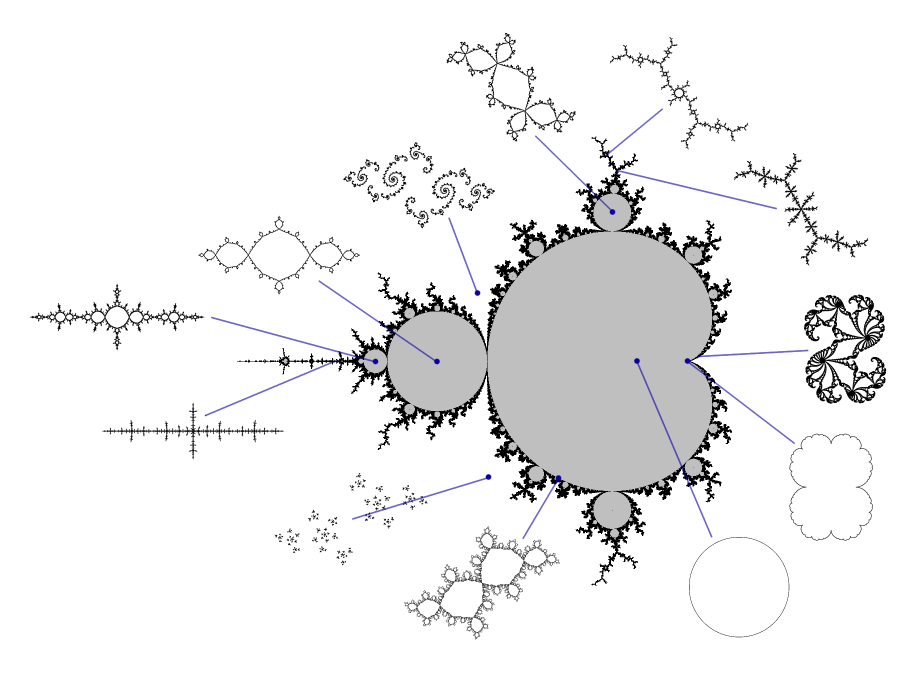
\includegraphics[width=0.5\textwidth]{mandel.png}
    \caption{\label{fig:mandel} Ensemble de Mandelbrot} 
\end{figure}

En zoomant on constate la dimension fratacle, un patterne qui se répète a l'infini.

\section{Fractale d'un diagramme de bifurcation}
Les fractales s'appliquent nottamment à la fonction logistique, plus précisément à son diagramme de bifurcation. On peut en effet aperçevoir une répétition lorsque nous zoomons aux alentours de $3,83$. Il y a un retour à l'ordre dans le comportment chaotique de cette fonction, avec un retour d'oscillation entre trois valeurs.
\begin{figure}[!ht]
    \begin{center}
        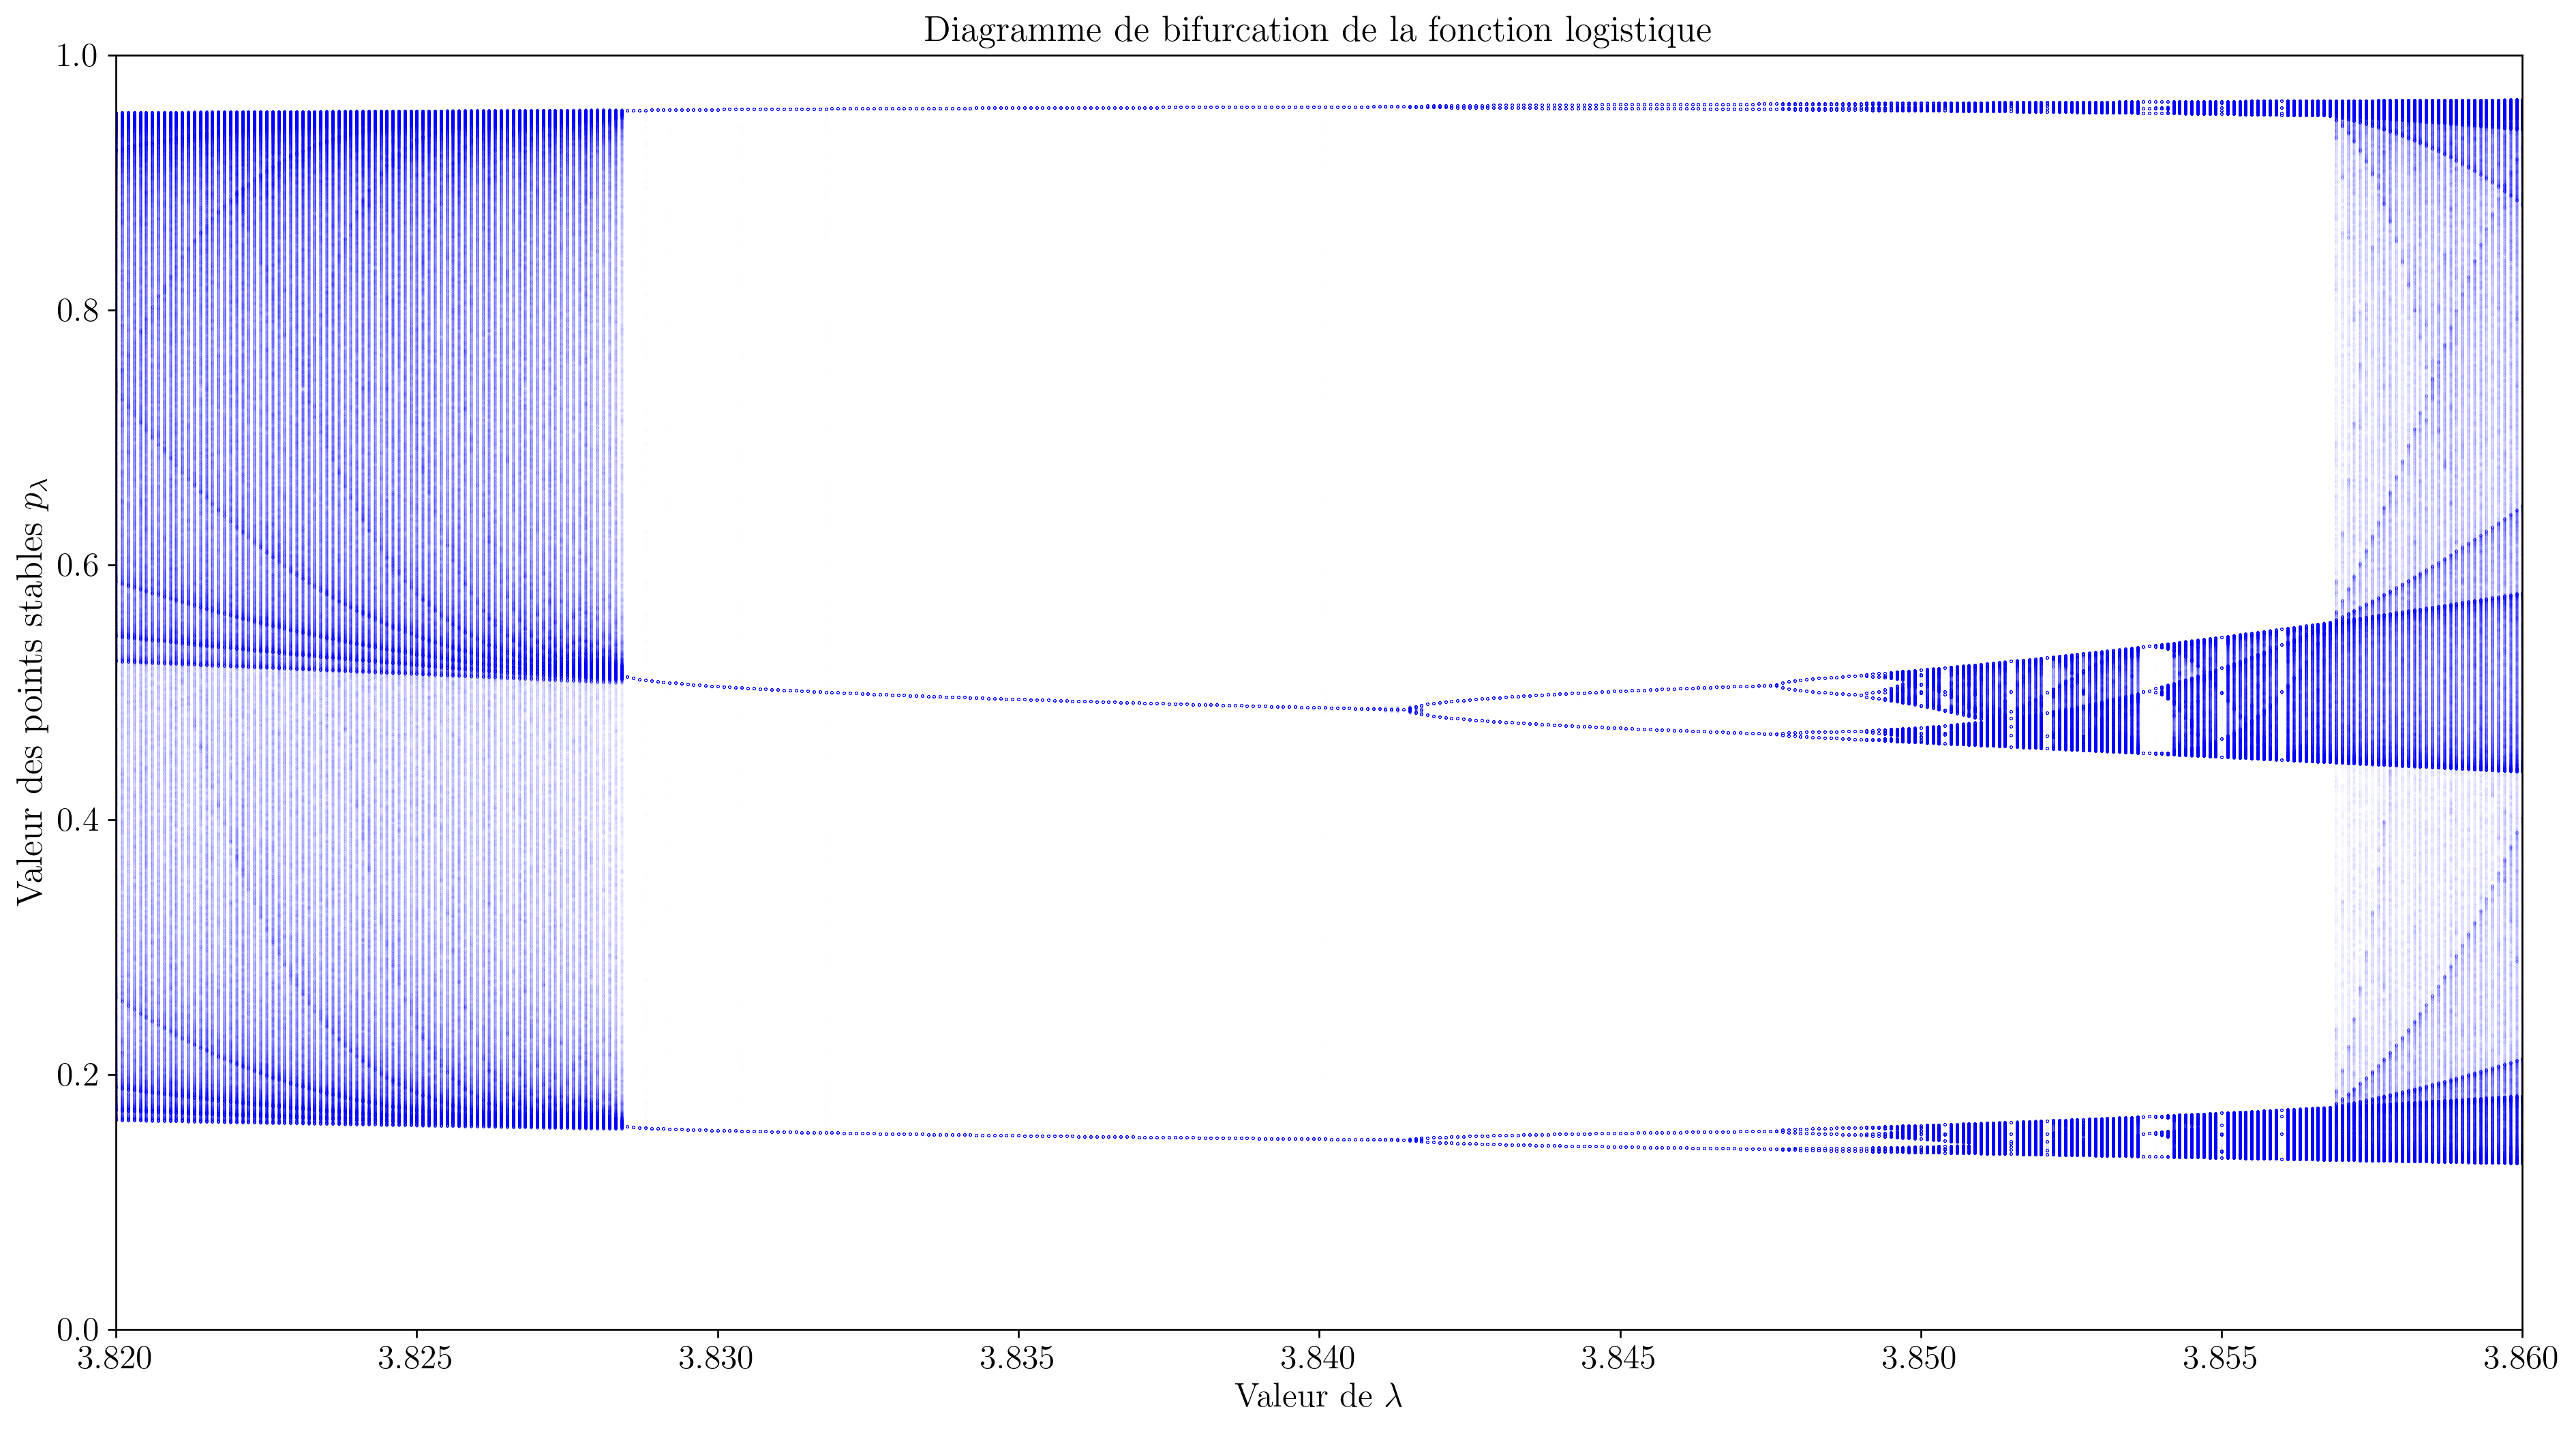
\includegraphics[width=\textwidth]{bifurcation_zoom.png}
    \end{center}
    \caption{\label{fig:bifurcation_zoom}Diagramme de bifurcation de la fonction logistique (agrandissement)}
\end{figure}
\section{Fratacle de l'attracteur de Lorenz}
Le cas de l'attracteur de Lorenz est particulier en ce qui concerne les fractales, car ça dimension fractale n'est pas directement observable sur sa représentation graphique, la première preuve de sa dimension fractale à été faite purement mathématiquement et sa première observation a été possible en traçant l'attracteur et en conservant 100 chiffre apès la virgule.